\documentclass[english]{article}
\usepackage[T1]{fontenc}
\usepackage[latin1]{inputenc}
\usepackage{a4}
\usepackage{amsmath}
\usepackage{babel}
\usepackage{times}
\usepackage{pslatex}
\usepackage{InsightMarkup}
\usepackage[pdftex]{graphicx}
\usepackage[bookmarksnumbered,colorlinks=true,pdftitle={},pdfauthor={Jordi Inglada},pdfsubject={},pdfkeywords={}]{hyperref}
\usepackage{fancyhdr}
\usepackage[normalem]{ulem}
\usepackage{afterpage}
\usepackage{rotating}
%\pagestyle{fancy}
\input epsf

% Define where in the disk is the Insight source tree 
% \def\ITKSOURCEDIR{}
% THOMAS
\def\ITKSOURCEDIR{/ORFEO/thomas/ORFEO-TOOLBOX/otb/OTB}
\graphicspath{{/ORFEO/thomas/ORFEO-TOOLBOX/otb/OTB-Documents/SoftwareGuide/Art/}{/ORFEO/thomas/ORFEO-TOOLBOX/otb/OTB-Documents/SoftwareGuide/Art/}}
\def\bibtexdatabasepath{/ORFEO/thomas/ORFEO-TOOLBOX/otb/OTB-Documents/SoftwareGuide/../Latex/Insight}


% Define command to make reference to on-line Doxygen documentation
\newcommand{\doxygen}[1]{
\href{http://www.itk.org/Doxygen/html/classitk_1_1#1.html}{\code{itk::#1}}}  

% Define command to make reference to on-line Doxygen documentation
\newcommand{\subdoxygen}[2]{
\href{http://www.itk.org/Doxygen/html/classitk_1_1#1_1_1#2.html}{\code{itk::#1::#2}}}  

% Define command for the standard comment introducing classes with similar functionalities
\newcommand{\relatedClasses}{
\textbf{The following classes provide similar functionality:}}




\usepackage{mdwtab}

\usepackage[normal]{subfigure}
\newcommand{\goodgap}{%
	\hspace{\subfigtopskip}%
	\hspace{\subfigbottomskip}}

\def\rit{\hbox{\it I\hskip -2pt R}}
\def\nit{\hbox{\it I\hskip -2pt N}}
\def\cut{\hbox{\it l\hskip -5.5pt C\/}}
\def\zit{\hbox{\it Z\hskip -2pt Z}}
\def\qit{\hbox{\it l\hskip -5.5pt Q}}


\def\BibTeX{{\rm B\kern-.05em{\sc i\kern-.025em b}\kern-.08em
    T\kern-.1667em\lower.7ex\hbox{E}\kern-.125emX}}


\begin{document}

\title{IDL/ENVI Bindings for the ORFEO Toolbox}
\author{OTB Development Team}


\maketitle

\tableofcontents


\section{Introduction}

This documentation is the result of a cooperation between the CNES (OTB developers) and ITT France (IDL/ENVI developers). Its aim to explain step by step how to wrap an OTB processing chain in IDL. First we describe how to create from OTB functions a dynamic library that can be called by an IDL function, then we show how to include such a function in an ENVI graphical user interface, GUI.

The procedures presented here were tested on Windows platforms (with Visual C++) and Linux machines (with GCC). Most of GUIs were created using ENVI tools.

\section{IDL Binding creation overview}

To be able to use OTB classes from within IDL or ENVI, the main requirement is to translate variables from one space to the other one. Few steps are necessary to create the interface for each OTB class you want to use. Several files need to be created as shown on Fig.~\ref{fig:overview}.

\begin{figure}[htp]
     \centering
      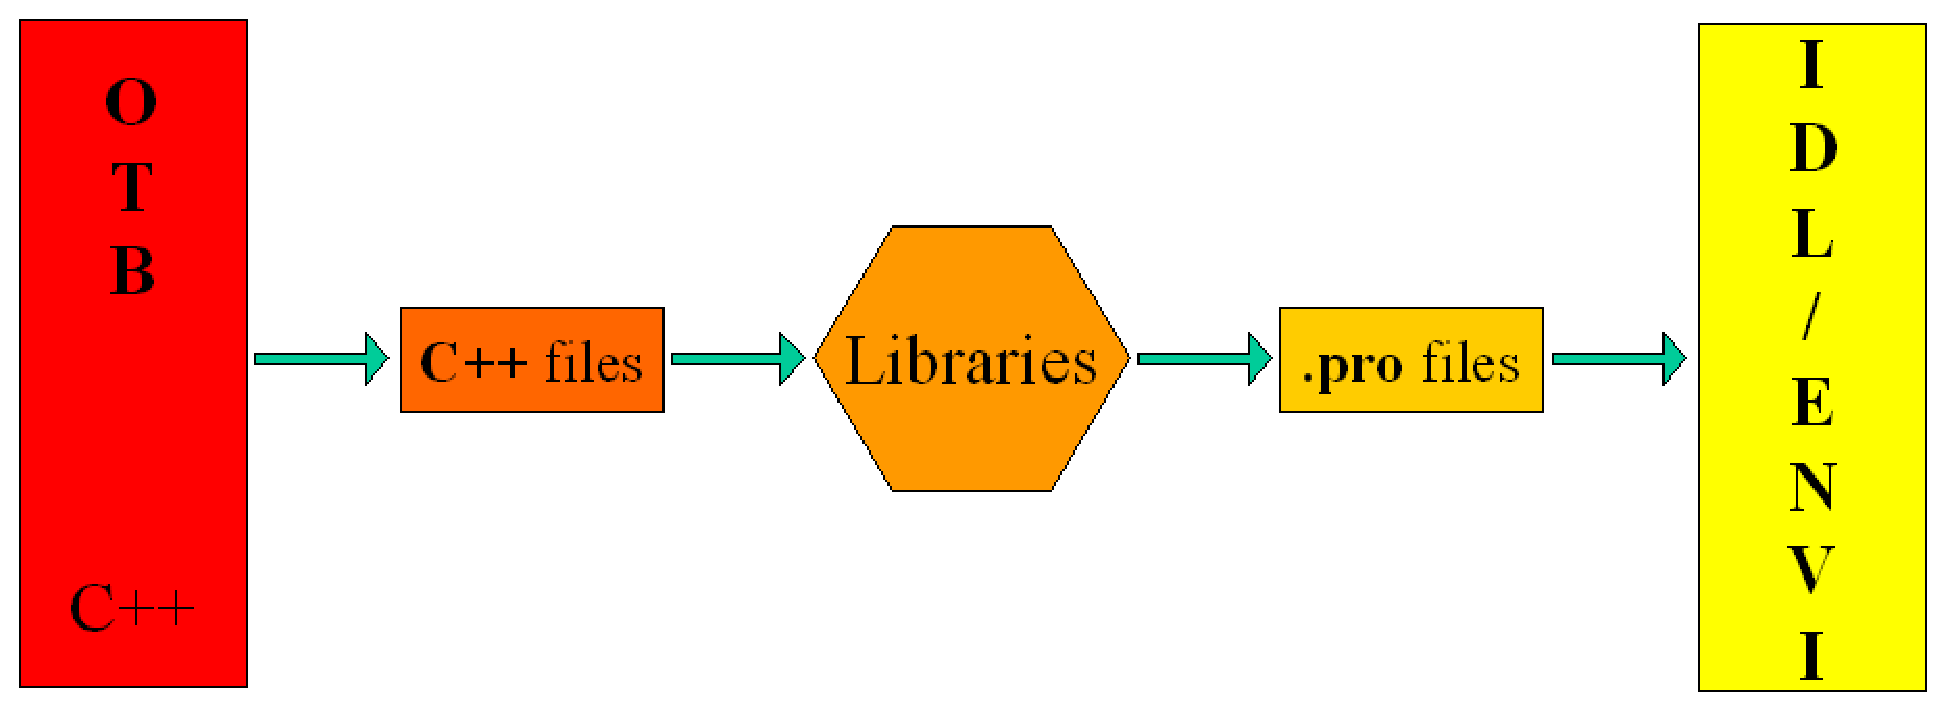
\includegraphics[width=8cm]{intro.eps}
      \caption{Overview of the binding process}\label{fig:overview}
\end{figure}

As the diagram shows it, the mechanism is simple. A layer is added to call OTB main with IDL inputs and ouputs data, executable is created and finally an IDL mecanism will create IDL routines that will use our OTB main.
First we will see how to create the project in section~\ref{buildProject}. Then we will see how to wrap a simple OTB main (Canny filter) in section~\ref{canny}, and later a complete explanation of
the C++ (section~\ref{cfiles}) and IDL files contents will be studied (section~\ref{idlfiles}) . At last, we will see how to integer those new IDL routine in the ENVI GUI (section~\ref{envi}).

\section{How to Build the Project:\\ CMake and CMakeList}
\label{buildProject}
In this section, the way to build a CMake file and to compile will be described.
Before going further, please check that the OTB is compiled on your computer.
To be compatible with the following PROCEDURES, your tree folders has to look like this:
\begin{itemize}
\item BINDING\_IDL/Binaries: where your .exe will be generated.
\item BINDING\_IDL/Code: where your sources are stored.
\end{itemize}

The \code{Code} folder can contain as many subfolders as you want. This allows you to organize your work space. The \code{Code} folder shipped along with this 
documentation contains a \code{Sources} folder where we put the C++ files while IDL files are stored in \code{IDLSources}. This documentation will not detail every lines of these files and it is necessary to start from the source example.

The \code{CMakeLists.txt} file located in the \code{Code} folder will take care of the CMake GUI and the compilation.

First, try to compile the binding example without any change to check if all tools are available. Launch the ccmake process from the BINDING\_IDL/binaries directory. It will ask you the path to the OTB exe directory 
(\/otb\-build/OTB) and paths to IDL source and binaries (located in your IDL folder):

\begin{itemize}
\item \code {IDL\_INCLUDE\_DIRS} that targets the IDL export includes. The path targets the IDL tree directory that contains export files (for example \code {usr/local/rsi/idl\_vXX/external/include}).
\item \code {IDL\_LIBRARY\_DIRS} that targets an IDL tree directory taht contains the IDL binaries (for example \code {usr/local/rsi/idl\_vXX/bin/bin.linux.x86}, for Linux 64bits target  \code{bin.linux.x86\_64}).
\end{itemize}

Once the cmake has generated its file, you can go to the binaries folder and compile.

Few things you should be aware when you are adapting the example to suit your needs: pay attention to add for each subfolder the following line in the \code{Code/Sources/CMakeLists.txt} file:\\
\code{SUBDIRS(ExampleDir)}\\
You'll also need to add in the \code{Code/CMakeLists.txt} file the following lines:
\code{\$\{OTB\-IDL\_BINARY\_DIR\}/Sources/ExampleDir}\\
\code{\$\{OTB\-IDL\_SOURCE\_DIR\}/Sources/ExampleDir}\\


Then the compiler will know that subfolders exist.
 
This is the tree folder:
\begin{verbatim}
Binaries
Code
        CMakeLists.txt
        Sources
                CMakeLists.txt
                Base
                    CMakeLists.txt
                Example1
                    CMakeLists.txt
        IDLSources
\end{verbatim}
 
In each subfolder, create a new CMakeLists.txt including the following lines (as the file Sources/Example1/CMakeLists.txt):
\begin{itemize}
\item The first one to gather the non-templated classes source (.cpp or .cxx) contained in the folder:\\ 
  \code {FILE(GLOB subdir1\_SRCS ``*.cxx'')}
\item The second to create a library using the declared source code:\\
  \code{ADD\_LIBRARY(libsubdir1 \${subdir1\_SRCS})}
\item The third to link this new library with the needed others one (that contain the include files) \textbf{and with the IDL lib}:\\
\code {TARGET\_LINK\_LIBRARIES (libName OTBCommon OTBBasicFilters OTBIO otbsvm \textbf{idl})}\\ 
\end{itemize}

\code{\textbf{Example:}}\\
      Here, we decide to create the example \code{Code/Sources} in the folder \code{Example1}.\\
      This is the contents of the \code{CMakeLists.txt file}:\\
\begin{verbatim}
      # Sources of non-templated classes.
      FILE(GLOB OTBIDLExample1_SRCS "*.cxx")
      ADD_LIBRARY(OTBIDLExample1 ${OTBIDLExample1_SRCS})
      TARGET_LINK_LIBRARIES (OTBIDLExample1 OTBCommon OTBBasicFilters OTBIO otbsvm idl)
\end{verbatim}


\section{A complete simple example : Canny filter}
\label{canny}
Here we'll present a simple example of OTB wrapping for IDL.
A canny filter has 2 parameters : input and output image name.
The complete example can be found in the tree example : \code{Code/Sources/Example1/idl\_otbcannyfilter.h} and \code{Code/Sources/Example1/idl\_otbcannyfilter.cxx}
\subsection{C++ files}
\subsubsection{.h and .cxx}
Let's start with the \code{.h}. To avoid multiple definitions, a \code{ifndef/defined} bloc has to be written.
The \code{idlotbdef.h} file has to be included, it contains usefull macros.
Finally, we declare the main using the macro \code{ORFEOANDIDL\_API} that will allow the IDL transcription.
Note that \code{void} indicates the fuction doesn't return anything. The created image is written in the main.
\code{IDL\_VPTR} is a tab containing the IDL inputs of the function 
\begin{verbatim}
    #ifndef _idlotbcannyfilter_h
    #define _idlotbcannyfilter_h

    #include "idlotbdef.h"

    ORFEOANDIDL_API void otbcannyfilter(int argc, IDL_VPTR argv[], char *argk);

    #endif
\end{verbatim}
\subsubsection{idl\_load.cxx}
Now the .cxx file.\\
First classical includes:
\begin{verbatim}
    #include "idl_otbcannyfilter.h"

    #include "otbImageFileReader.h"
    #include "otbImageFileWriter.h"
    #include "otbImage.h"
    #include "itkCastImageFilter.h"
    #include "itkRescaleIntensityImageFilter.h"
    #include "itkCannyEdgeDetectionImageFilter.h"
\end{verbatim}
Then the function corpus starting with the function declaration:
\begin{verbatim}
ORFEOANDIDL\_API void otbcannyfilter(int argc, IDL\_VPTR argv[], char *argk)
{
\end{verbatim}
We transform function inputs (that are IDL datas) into C++ variables (here, input and ouput file name).
First we instanciate \code{char*} that will contain input value. Quote that \code{char*} are used because inputs are strings.
\begin{verbatim}
  static char inputFilename[MAX_LENGTH];
  static char outputFilename[MAX_LENGTH];
\end{verbatim} 
Then will fill our C++ variables using memory copy.\\
First we check the IDL input is not empty, then we copy its value in our C++ variable.
\begin{verbatim}
  if (argv[0]->value.str.s != NULL)
    strcpy(inputFilename, argv[0]->value.str.s);
  
  if (argv[1]->value.str.s != NULL)
		strcpy(outputFilename, argv[1]->value.str.s);
\end{verbatim}
Now we can work with our variables, using it in a classical C++ way.
\begin{verbatim}
  float variance = 2;
  typedef unsigned char    CharPixelType;  //  IO
  typedef double           RealPixelType;  //  Operations
  const   unsigned int     Dimension = 2;
  
  typedef otb::Image<CharPixelType, Dimension>                             CharImageType;
  typedef otb::Image<RealPixelType, Dimension>                             RealImageType;
  typedef otb::ImageFileReader< CharImageType>                             ReaderType;
  typedef otb::ImageFileWriter< CharImageType>                             WriterType;
  typedef itk::CastImageFilter< CharImageType, RealImageType>              CastToRealFilterType;
  typedef itk::RescaleIntensityImageFilter<RealImageType, CharImageType >  RescaleFilter;
  typedef itk::CannyEdgeDetectionImageFilter<RealImageType, RealImageType> CannyFilter;
  
  //Setting the IO
  ReaderType::Pointer           reader      = ReaderType::New();
  WriterType::Pointer           writer      = WriterType::New();
  CastToRealFilterType::Pointer toReal      = CastToRealFilterType::New();
  RescaleFilter::Pointer        rescale     = RescaleFilter::New();
  //Setting the ITK pipeline filter
  CannyFilter::Pointer          cannyFilter = CannyFilter::New();
  
  reader->SetFileName( inputFilename  );
  writer->SetFileName( outputFilename );
  
  //The output of an edge filter is 0 or 1
  rescale->SetOutputMinimum(   0 );
  rescale->SetOutputMaximum( 255 );
  
  toReal->SetInput( reader->GetOutput() );
  
  cannyFilter->SetInput( toReal->GetOutput() );
  cannyFilter->SetVariance( variance );
  rescale->SetInput( cannyFilter->GetOutput() );
  writer->SetInput( rescale->GetOutput() );
  
  writer->Update();
}
\end{verbatim}
Now the C++ main is done, you need to register the function into IDL. That's what \code{idl\_load.cxx} does.
\\
First, add the include:
\begin{verbatim}
#include "idl_otbcannyfilter.h"
\end{verbatim}
In the \code{IDL\_Load()} method we add the function call.\\
Remind that the IDL routines will take onlytwo arguments (input and ouput file name), this explain the "2" in the following extracted code and let's start with the IDL routine definition:
\begin{verbatim}
	IDL_SYSFUN_DEF2 procedure_canny[] = {  
	{ (IDL_SYSRTN_GENERIC)otbcannyfilter, "OTBCANNYFILTER", 2, 2, 0, 0},  
	}; 
\end{verbatim}
This is generic lines. From a new treatment to an other, only name and number of inputs changes.\\
Now the method return:
\begin{verbatim}
    return IDL_SysRtnAdd(procedure_canny, FALSE,   
	IDL_CARRAY_ELTS(procedure_canny));
\end{verbatim}

We've finished with the C++ part. Now, you can compile the project and then have a look to the IDL part with the \code{resoreroutines.pro} file.

\subsection{IDL Function creation}
The \code{resoreroutines.pro} file creates a IDL routines from our C++ function.
Only one line need to be added. This line precises, the created IDL routines name, the path to the lib that contains the exe made from our C++ main and tha maximum and miunimum number of arguments the IDL routine will takes.
\begin{verbatim}
     LINKIMAGE, 'otbcannyfilter', file_dllExample1, 0, MAX_ARGS = 2, MIN_ARGS = 2
\end{verbatim}

Here, \code{file\_dllExample1} target \code{../Binaries/bin/libOTBIDLExample.1.so} because the canny function was made and compile in the Example1 directory.
Note taht when you call the restoreroutines routine, you have to precise as argument the path to your binaries (here \code{../Binaries/bin/}).\\
Congratulation, IDL knows now the OTBCANNYFILTER routine.\\
It can be called from IDL with the following line:
\emph {OTBCANNYFILTER, "InputImage", "OutputImage"}

After this simple example, let's see more complete (and complexe) explanations of the wrapping mecanism.

\section{C++ processing functions}
\label{cfiles}
\subsection{Input and Output Types}
To make things easy, we chose to create one C++ file for each wanted IDL function. Those files are \code{.h} and \code{.cxx} files stored in \code{Code/Sources/Example1} in the example tree.

To avoid multiple definitions due to links between excutables, an ifndef/define bloc has to be writen:\\
\code{\#ifndef \_myfunction\_h}\\
\code{\#ifndef \_myfunction\_h}\\
And, at the end of the \code{.h} file:
\code{\#endif}\\
Besides the header files needed for the code compilation, the following file has to be included: \code{idlotbdef.h}. This file is stored in \code{Code/Sources/Base} and included in the package and contains the definition of the \code{ORFEOANDIDL\_API} macro defined below in this document.

The C++ functions have to be defined as follows:\\
\code {ORFEOANDIDL\_API void OTBToIDLFunction(\textbf {int argc, IDL\_VPTR argv[], char *argk})}\\
Where:
\begin{itemize}
    \item \code{argc} is the number of inputs;
    \item \code{argv[]} is an IDL pointer (\code{IDL\_VPTR}) to a \code{char *} array;
    \item \code{argk} is a char pointer.
\end{itemize}
\code{IDL\_VPTR} is an idl pointer that can return any kind of IDL variable.
For the outputs, two solutions can be used :
\begin{itemize}
\item The output is void (the image is stored in the class): \\ 
\code {\textbf {ORFEOANDIDL\_API void} OTBToIDLFunction(int argc, IDL\_VPTR argv[], char *argk)}.\\
  The output name is given as an element of the \code{argv[]} array. The corresponding IDL routine is a \textbf{function}.
\item The output is not void, an IDL pointer is used: \\ 
\code {\textbf {ORFEOANDIDL\_API IDL\_VPTR} OTBToIDLFunction(int argc, IDL\_VPTR argv[], char *argk)}.\\
  This pointer can point to any kind of IDL variable. The corresponding IDL routine is a \textbf{procedure}.
\end{itemize}
\code{ORFEOANDIDL\_API} is a C++ macro that ensures that the symbol name associated to the compiled function will be exactly the same as the function name. Without it, 
on Linux some extra characters are added to the name. In this case, when the \code{.pro} file is compiled, an error occurs since the symbol can't be found. \\
\\
\textbf{Example:}\\
      We show here how to add an IDL function that performs image ortho rectification. For additional explanation of the algorithm, please refer to the OTB Software Guide.

      In \code{idl\_otborthorectification.h}, the function is defined as:
\begin{verbatim}
    #ifndef _idlotborthorectification_h
    #define _idlotborthorectification_h

    #include "idlotbdef.h"

    ORFEOANDIDL_API void otborthorectification(int argc, IDL_VPTR argv[], char *argk);

    #endif

\end{verbatim}

Once the signature of the functions is written, we need to make the link IDL/OTB and OTB/IDL.

\subsection{How to wrap variables?}
\subsubsection{IDL to OTB : IDL to C variable wrapping}
Two cases appear: link a string or other type (double, int, float, array, etc.)

\begin{itemize}
\item For a string:\\
  The variable is declared:\\ 
  \code{static char inputImageFileName[MAX\_LENGTH]}\\
  and instanciated with the IDL input value:\\ \code{strcpy(inputImageFileName, argv[0]->value.str.s)}\\
\item In the other cases:\\
  First, we declare and initialize the variable:\\ \code{double value = 0.}\\
  and then the idl pointer is used to instanciate the OTB variable:\\ \code{double value = argv[0]->value.d}\\
\end{itemize}
Those two variables are now initialized and be can used in the OTB code (\code{filter->SetInputName(inputImageFileName)} for example).
\\
\\
\underline{Nota Bene:} Please note, that passing an \code{IDL\_VPTR} to an image as argument is possible but not recommended, passing the image path is more efficient.

\subsubsection{OTB to IDL : C to IDL variables wrapping}
If the user has decided that the C++ function doesn't have to return anything, nothing else has to be done. Otherwise (the C++ function is an IDL procedure and  has to return an IDL pointer), the inverse mechanism has to be implemented, that is to say, transform an OTB variable in an IDL variable. This is the way to do that :
\begin{itemize}
  \item The output is an image:
    \begin{itemize}
    \item Declare the output:\\ \code{IDL\_VPTR IDLOutput};
    \item Create a pointer to the input image:\\ \code{IDL\_VPTR IDLSrc = IDL\_CvtDbl(1, \&argv[0])};
    \item Allocate the output and create a pointer to its first byte:\\ \code{char *firstByte = (char *)IDL\_VarMakeTempFromTemplate(IDLSrc, IDLSrc->type, NULL, \&IDLOutput, true)};
    \item Store the output image:\\ \code{double* pData = (double *)filter->GetOutput()->GetBufferPointer()};
    \item Fill the IDL output with the output image:\\ \code{memcpy((char *)firstByte, (char *)pData, IDLSrc->value.arr->arr\_len)};
    \end{itemize}
  \item The output is not an image (double, int, array, etc.):
    \begin{itemize}
    \item Declare the output:\\ \code{IDL\_VPTR IDLOutput};
    \item Allocate the output:\\ \code{IDLOutput->Gettmp()};
    \item Declare the output variable type:\\ \code{IDLOutput->type = IDL\_TYP\_DOUBLE} for a double;
    \item And fill the output:\\ \code{IDLOutput->value.d = filter->GetOutputValue()} if the pointer points to a double.
    \end{itemize}
\end{itemize}


The user can now write his OTB processing function.
\\
\\
\textbf{Example:}\\
      In \code{idl\_otborthorectification.cxx}:\\
      Include declaration:\\
\begin{verbatim}
      #include "otbImage.h"
      #include "otbVectorImage.h"
      #include "otbImageFileReader.h"
      #include "otbStreamingImageFileWriter.h"
      #include "otbPerBandVectorImageFilter.h"
      #include "otbOrthoRectificationFilter.h"
      #include "otbMapProjections.h"
\end{verbatim}

      \textbf{Function declaration:}\\
\begin{verbatim}
      ORFEOANDIDL_API void otborthorectification(int argc, IDL_VPTR argv[], char *argk)
      {
      //Inputs casting
      //Inputs declaration
      static char inputFilename[MAX_LENGTH];
      static char outputFilename[MAX_LENGTH];
      static unsigned int utmZone= 1;
      static char hemisphere[MAX_LENGTH];
      static char xGroundUL[MAX_LENGTH];
      static char yGroundUL[MAX_LENGTH];
      static double xGroundSampling = 1.;
      static double yGroundSampling = 1.;
      static long unsigned int xSize=500;
      static long unsigned int ySize=500;
\end{verbatim}

      \textbf{Input initialization:}\\
\begin{verbatim}
      if (argv[0]->value.str.s != NULL)
      strcpy(inputFilename, argv[0]->value.str.s);
      if (argv[1]->value.str.s != NULL)
      strcpy(outputFilename, argv[1]->value.str.s);
      utmZone = static_cast<unsigned int>(argv[2]->value.d);
      if (argv[3]->value.str.s != NULL)
      strcpy(hemisphere, argv[3]->value.str.s);
      if (argv[4]->value.str.s != NULL)
      strcpy(xGroundUL, argv[4]->value.str.s);
      if (argv[5]->value.str.s != NULL)
      strcpy(yGroundUL, argv[5]->value.str.s);
      xSize = static_cast<long unsigned int>(argv[6]->value.d);
      ySize = static_cast<long unsigned int>(argv[7]->value.d);
      xGroundSampling = argv[8]->value.d;
      yGroundSampling = argv[9]->value.d;
\end{verbatim}
Note that even for \code{unsigned int} input, we work with \code{IDL\_VPTR} of double type. This was made because the widget used for the \code{IDL GUI} returns a double. In other cases, a simple \code{utmZone = argv[2]->value.ui} would be correct.\\

      \textbf{The C++ code of the function:}\\
\begin{verbatim}
      typedef otb::Image<unsigned char, 2>                    CharImageType;
      typedef otb::Image<unsigned int, 2>                     ImageType;
      typedef otb::VectorImage<unsigned int, 2>               VectorImageType;
      typedef otb::ImageFileReader<VectorImageType>           ReaderType;
      typedef otb::StreamingImageFileWriter<VectorImageType>  WriterType;
      typedef otb::UtmInverseProjection                       utmMapProjectionType;
      typedef otb::OrthoRectificationFilter<ImageType, ImageType, utmMapProjectionType>              OrthoRectifFilterType;
      typedef otb::PerBandVectorImageFilter<VectorImageType, VectorImageType, OrthoRectifFilterType> PerBandFilterType;

      ReaderType::Pointer            reader            = ReaderType::New();
      WriterType::Pointer	       writer            = WriterType::New();
      OrthoRectifFilterType::Pointer orthoRectifFilter = OrthoRectifFilterType::New();
      utmMapProjectionType::Pointer  utmMapProjection  = utmMapProjectionType::New();
      PerBandFilterType::Pointer     perBandFilter     = PerBandFilterType::New();

      reader->SetFileName(inputFilename);
      writer->SetFileName(outputFilename);
      utmMapProjection->SetZone(utmZone);
      utmMapProjection->SetHemisphere(*(hemisphere));
      orthoRectifFilter->SetMapProjection(utmMapProjection);
      perBandFilter->SetFilter(orthoRectifFilter);
      perBandFilter->SetInput(reader->GetOutput());

      ImageType::IndexType start;
      start[0]=0;
      start[1]=0;
      orthoRectifFilter->SetOutputStartIndex(start);
      ImageType::SizeType size;
      size[0]=xSize;
      size[1]=ySize;
      orthoRectifFilter->SetSize(size);
      ImageType::SpacingType spacing;
      spacing[0]=xGroundSampling;
      spacing[1]=yGroundSampling;
      orthoRectifFilter->SetOutputSpacing(spacing);
      ImageType::PointType origin;
      origin[0]=strtod(xGroundUL, NULL);
      origin[1]=strtod(yGroundUL, NULL);
      orthoRectifFilter->SetOutputOrigin(origin);

      writer->SetInput(perBandFilter->GetOutput()); 	
      writer->SetTilingStreamDivisions();
      writer->Update();
\end{verbatim}

\subsection{The link IDL-OTB}
To be transformed into an IDL function, you have to declare the C++ functions that need to be exported, the name of the IDL function 
that will be generated in IDL, the minimal number of inputs, the maximal number of inputs and the minimal and maximal number of keywords. \\
This mechanism is performed by the \code{idl\_load.cpp} C++ function.
First you have to add a reference to your function using an include:\\
\code{\#include "OTBToIDLFunction.h"}
\\
After that, you need to complete the \code{idl\_load.cpp} code to declare your function, two cases appear:
\begin{itemize}
\item The C++ function corresponds to a IDL procedure:
  \begin{itemize}
  \item Add the declaration (in the definition corpus):\\
    \code{IDL\_SYSFUN\_DEF2 procedure\_functionname[]=\{\{(IDL\_SYSRTN\_GENERIC)otbfunctionname, "OTBFUNCTIONNAME", minInput, maxInput, minKeyword, maxKeyword\}\}}
  \item Add the return (in the return corpus):\\
    \code{IDL\_SysRtnAdd(procedure\_functionname, \textbf{FALSE}, IDL\_CARRAY\_ELTS(procedure\_functionname))}
  \end{itemize}
\item The C++ function corresponds to an IDL function:
  \begin{itemize}
  \item Add the declaration (in the definition corpus):\\
    \code{return IDL\_SYSFUN\_DEF2 function\_functionname[] = \{\{ (IDL\_SYSRTN\_GENERIC)otbfunctionname, "OTBFUNCTIONNAME", minInput, maxInput, minKeyword, maxKeyword\}\}}
  \item Add the return (in the return corpus):\\
    \code{return IDL\_SysRtnAdd(function\_functionname, \textbf{TRUE}, IDL\_CARRAY\_ELTS(function\_functionname))}
  \end{itemize}
\end{itemize}

\textbf{Example:}\\
      In the \code{idl\_load.cpp} file, add the include:\\
      \code{\#include "idl\_otborthorectification.h"}\\

      In the definition corpus area:\\
      orthorectification function declaration:\\
\begin{verbatim}
      IDL_SYSFUN_DEF2 procedure_orthorectif[] = {
      { (IDL_SYSRTN_GENERIC)otborthorectification, "OTBORTHORECTIFICATION", 10, 
        10, 0, 0},
      };
\end{verbatim}
      In return corpus area: \\
\begin{verbatim}
      return IDL_SysRtnAdd(procedure_orthorectif, TRUE,
      IDL_CARRAY_ELTS(procedure_orthorectif));
\end{verbatim}

\underline{N.B:}
 \begin{itemize}
\item The name definition (\code{procedure\_functionname} or \code{function\_functionname}) doesn't have any importance, we chose those ones to be as clear as possible.
\item If several C++ functions are declared, write only one \code{return} but separate its elements with \code{\&\&}:\\
      \code{return IDL\_SysRtnAdd(procedure\_function1, TRUE, IDL\_CARRAY\_ELTS(procedure\_function1)) \textbf{\&\&} IDL\_SysRtnAdd(procedure\_function2, FALSE, IDL\_CARRAY\_ELTS(procedure\_function2));} \\
\end{itemize}


\section{IDL Function creation}
label{idlfiles}
\subsection{restoreroutines.pro}
This file integrates in IDL the function included in the shared library. Its location doesn't have any importance, but it is better to gather all \code{.pro} files in the same folder.
We arbitrary chose to put them in \code{Code/IDLSources}.
The aim of create an IDL routine from the created excecutable. For this you it needs to know the localization of the executable. This path has to be given as input to the routine.
Pay attention to the fact that each created libraries contains only the binaries for the C++ functions of the directory used to generated the bin.
Thus you may need to declare multiple file path (one for each interesting lib).

\begin{itemize}
\item The C++ function corresponds to a IDL procedure:\\
  \code{LINKIMAGE, 'otbfunctionname', file\_dll, 1, /FUNCT, MAX\_ARGS = 4, MIN\_ARGS = 4}
\item The C++ function corresponds to a IDL function:\\
  \code{LINKIMAGE, 'otbfunctionname', file\_dll, 0, MAX\_ARGS = 4, MIN\_ARGS = 4}
\end{itemize}
IDL knows now our function under the name \code{OTBFUNCTIONNAME}.\\

\code{\textbf{Example:}}\\
      In the \code{restoreroutines.pro} file:\\
\begin{verbatim}
      LINKIMAGE, 'otborthorectification', file_dllExample1, 0, MAX_ARGS = 10, MIN_ARGS = 10
\end{verbatim}

Here file\_dllExample1 targets Example1 library.
IDL knows now our function under the name \code{OTBORTHORECTIFICATION}, and it must have 10 input arguments. The function can used like taht, but can be included too in a IDL GUI.
That's the aim of the following section.\\



\subsection{orfeo\_function.pro}
A specific file can be made to link the inputs/outputs of the function with GUIs, etc.
The function is called using :\\
\code{OTBFUNCTIONNAME(arg1, arg2, arg3, ...)}
\\
\textbf{Example:}\\
      Note that this example creates an IDL GUI, a one line IDL routine which gives its arguments to the IDL orthorectification function works as well.\\
      In the \code{orfeo\_orthorectificationfilter.pro} file:\\
\begin{verbatim}
      PRO orfeo_orthorectificationfilter, ev
      ; Select an input file :
      fileIN = ENVI_PICKFILE(TITLE = "Select an input file")
      IF fileIN EQ '' THEN $
      MESSAGE, "You must select an input file"
      ENVI_OPEN_FILE, fileIN, R_FID = fid
      ENVI_FILE_QUERY, fid, NB = nb
      ENVI_DISPLAY_BANDS, REPLICATE(fid, nb), INDGEN(nb)

      fileOut = ENVI_PICKFILE(TITLE = "Select an output file")
      IF fileOUT EQ '' THEN $
      MESSAGE, "You must select an output file"

      tlb = WIDGET_AUTO_BASE(title = 'Ortho Rectification filter parameters')

      p1 = WIDGET_PARAM(TLB, /AUTO_MANAGE, DT = 10, FIELD = 2, $
      PROMPT = 'UTM Zone:', UVALUE = 'UtmZone', DEFAULT = 31)
      p2 = WIDGET_STRING(TLB, PROMPT = 'Hemisphere:', UVALUE = 'Hemisphere', /auto, DEFAULT = 'N')
      p3 = WIDGET_STRING(TLB, PROMPT = 'X Ground UL:', UVALUE = 'XGroundUL', /auto, DEFAULT = '375000')
      p4 = WIDGET_STRING(TLB, PROMPT = 'Y Ground UL:', UVALUE = 'YGroundUL', /auto, DEFAULT = '4828100')
      p5 = WIDGET_PARAM(TLB, /AUTO_MANAGE, DT = 12, FIELD = 100, $
      PROMPT = 'X Size:', UVALUE = 'XSize', DEFAULT = 500)
      p6 = WIDGET_PARAM(TLB, /AUTO_MANAGE, DT = 12, FIELD = 100, $
      PROMPT = 'Y Size:', UVALUE = 'YSize', DEFAULT = 500)
      p7 = WIDGET_PARAM(TLB, /AUTO_MANAGE, DT = 10, FIELD = 2, $
      PROMPT = 'X ground Sampling:', UVALUE = 'XGroundSampling', DEFAULT = 0.6)
      p8 = WIDGET_PARAM(TLB, /AUTO_MANAGE, DT = 10, FIELD = 2, $
      PROMPT = 'Y ground Sampling:', UVALUE = 'YGroundSampling', DEFAULT = -0.6)

      res = AUTO_WID_MNG(TLB)

      ; Default values :
      IF res.accept EQ 0 THEN BEGIN
      res.UtmZone = 31.
      res.Hemisphere = "N"
      res.XGroundUL = 375000
      res.YGroundUL = 4828100
      res.XSSSize = 500
      res.YSSSize = 500
      res.XGroundSampling = 0.6
      res.YGroundSampling = -0.6
      END

      OTBORTHORECTIFICATION, fileIn, fileOut, $
      res.UtmZone , res.Hemisphere , res.XGroundUL , res.YGroundUL , $
      res.XSize , res.YSize , res.XGroundSampling , res.YGroundSampling 

      ; Read image :
      imageOut = READ_IMAGE(fileOut)
      ENVI_OPEN_FILE, fileOut, R_FID = fidout
      ENVI_FILE_QUERY, fidout, NB = nbout
      ENVI_DISPLAY_BANDS, REPLICATE(fidout, nbout), INDGEN(nbout)
      ENVI_ENTER_DATA, imageOut

      END
\end{verbatim}
This GUI opens a browser to select the input and output images and displays it. It opens the parameter selection box. The used functions are part of ENVI, thus, you have to launch ENVI in background to be able to compile the file. This last part shows how to call the IDL function with a GUI. Another solution is to insert the call in the ENVI GUI.


\section{Using OTB Routines in ENVI}
\label{envi}
This section aims to show the integration of OTB routines in the ENVI GUI.

Before going further, the user needs to move or copy his dynamic library : \code{.dll} or \code{.so} and \code{.dlm} (Dynamically Loadable Module) 
that contains the OTB routine into the folder  \code{...\\ITT\\IDL64\\bin\\bin.x86}.\\
The library has the same name as the OTB function and the binaries folder. For the following example, the \code{OTBTOUZIEDGEDECTOR} routine is needed.\\
In this part, three steps are described :
\begin{itemize}
    \item The modification of the main ENVI menu bar, in order to add some OTB options (the Touzi Edge Detector filter).
    \item The creation of a Graphical User Interface that allows getting the user parameters associated with the Touzi Edge Detector filter
    (two approaches are described : in \ref{enviapp}, a  purely ENVI  and in \ref{enviidlapp}, a  mixed IDL + ENVI  approach).
    \item The modification of the IDL path in order to include the paths to the routines mentioned in the previous step. 
\end{itemize}

\section{Modification of the ENVI menu bar} 

We present here how to modify the ENVI menu bar in order to add the entry \code{ORFEO Filters->Touzi edge detector}.
\begin{itemize}
    \item Open the text file \code{envi.men} located in \code{...\\ITT\\IDL64\\products\\envi44\\menu}.
    \item At the end of the file, add the lines below.
        \begin{verbatim}
                  0 {ORFEO Filters}
                  1 {Touzi edge detector} {not used} {simpleIDLGUI}
        \end{verbatim}
        \code{Level 0} means that the entry  \code{ORFEO Filters}  will belong to the main ENVI menu bar. 
        \code{Level 1} means that the entry  \code{Touzi edge detector} will belong to the menu  \code{ORFEO Filters}  and will appear right below it.
    \item  \code{simpleIDLGUI} is the name of the IDL routine that will be called when the option \code{Touzi edge detector} is selected .
    \item Save the \code{envi.men} text file (you should keep a copy of the original file).
    \item When ENVI will be launched next time, the main menu bar will be automatically modified, and will include a new \code{ORFEO Filters} entry.
\end{itemize}


\section{Creation of the graphical user interface}
We describe here how to create the graphical user interface that will be launched after selecting the  ORFEO Filters->Touzi edge detector  option. Two approaches are described:
 \begin{itemize}
    \item Building the GUI using exclusively ENVI widgets (requires basic knowledge of ENVI programming).
    \item Building the GUI using both ENVI and IDL widgets (requires very little knowledge of ENVI programming, 
        but good knowledge of IDL programming).
\end{itemize}

\subsection{ENVI approach}\label{enviapp}
In the example below, the GUI is developed using exclusively ENVI widgets. The main procedure is called \code{simpleENVIGUI}. 
and takes one input parameter (even if this parameter is not used in the routine). The routines \code{WIDGET\_AUTO\_BASE}, \code{WIDGET\_OUTF}, \code{WIDGET\_PARAM} 
and \code{AUTO\_WID\_MNG} correspond to ENVI routines. The parameters entered in the GUI by the user are automatically stored into the result structure. 
The fields from that structure are then passed as input parameters to the routine \code{OTBTOUZIEDGEDETECTOR} (this routine belongs to the Dynamically Loaded Module).
Finally, the input and output files are loaded into ENVI using the routine \code{ENVI\_OPEN\_FILE}.

The GUI should look like the figure~\ref{fig:fileselectiontest}.

\begin{figure}
\label{fileselectiontest}
\begin{center}
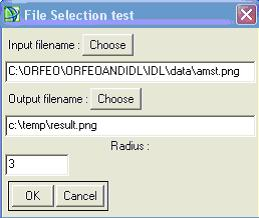
\includegraphics[width=7cm]{fileselectiontest.eps}
\caption{File selection}
\end{center}
\label{fig:fileselectiontest}
\end{figure}


\textbf{Example:}\\
      This is the source code for \code{simpleENVIGUI.pro} file:\\
\begin{verbatim}
      PRO simpleENVIGUI, ev

      ; Error handler :
      err = 0
      CATCH, err
      IF err NE 0 THEN BEGIN
            res = DIALOG_MESSAGE(!error_state.msg, /ERROR)
            res = DIALOG_MESSAGE(!error_state.msg, /ERROR)
            CATCH, /CANCEL
            RETURN
      END

      ; Create simple widgets :
      base = WIDGET_AUTO_BASE(TITLE = 'File Selection test')

      ; Select input file :
      wi = WIDGET_OUTF(base, UVALUE = 'inf', /AUTO, PROMPT = 'Input filename :')

      ; Select output file :
      wo = WIDGET_OUTF(base, UVALUE = 'outf', /AUTO, PROMPT = 'Output filename :', $
      DEFAULT = 'c:/temp/result.eps')

      ; Define radius :
      wRadius = WIDGET_PARAM(base, DT = 2, PROMPT = "Radius :", /AUTO, UVALUE = "Radius",  DEFAULT = 3)

      ; Auto manage :
      result = AUTO_WID_MNG(base)

      ; User hit Cancel button :
      IF result.accept EQ 0 THEN $
            RETURN

      ; Check values :
      IF ~FILE_TEST(result.inf) THEN $
            MESSAGE, "Invalid input filename"
      IF result.outf EQ '' THEN $
            MESSAGE, "Invalid output filename"

      ; Get widget values and do processing :
      WIDGET_CONTROL, /HOURGLASS
      ; Call TOUZI edge detector :
      OTBTOUZIEDGEDETECTOR, result.inf, result.outf, $
      FIX(result.radius)
      WIDGET_CONTROL, HOURGLASS = 0

      ; Load files into ENVI :
      ENVI_OPEN_DATA_FILE, result.inf
      ENVI_OPEN_DATA_FILE, result.outf

      END
\end{verbatim}

\subsection{ENVI+IDL approach}\label{enviidlapp}
In the example below, the GUI is developed using ENVI and IDL widgets. The widgets come from the IDL standard widget library, 
but the loading of the images into ENVI is performed using ENVI routines.

The GUI should look like the figure ~\ref{simpleidlgui}.

\begin{figure}
\label{simpleidlgui}
\begin{center}
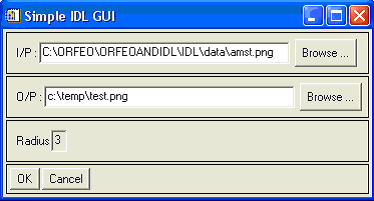
\includegraphics[width=7cm]{simpleidlgui.eps}
\caption{Simple IDL GUI}
\end{center}
\end{figure}

The source code contains two main routines:
\begin{itemize}
    \item The \code{simpleIDLGUI} routine actually builds the GUI.
    \item The  \code{simpleIDLGUI\_event} routine allows handling user events, i.e. to process all user interactions.
    \item The processing itself is performed when the user hits the \code{OK} button. The  \code{OTBTOUZIEDGEDETECTOR} routine is then called, while passing to it the required parameters.
    \item The loading of the data into ENVI is made by the \code{ENVI\_OPEN\_DATA\_FILE} routine.
\end{itemize}

\textbf{Example:}\\
      This is the source code for \code{simpleIDLGUI.pro} file:\\
\begin{verbatim}
      ; Main event handler :
      PRO simpleIDLGUI_event, ev

      ; Error handler :
      err = 0
      CATCH, err
      IF err NE 0 THEN BEGIN
            res = DIALOG_MESSAGE(!error_state.msg, /ERROR)
            CATCH, /CANCEL
            RETURN
      END

      ; Get state structure :
      WIDGET_CONTROL, ev.top, GET_UVALUE = pState

      ; Get user value :
      WIDGET_CONTROL, ev.id, GET_UVALUE = uval

      CASE uval OF
            "browseinput": BEGIN
                  strInputFile = DIALOG_PICKFILE()
                  IF ~FILE_TEST(strInputFile) THEN $
                        MESSAGE, "Invalid input filename"
                  WIDGET_CONTROL, (*pState).wInputFile, SET_VALUE = strInputFile
            END
            "browseoutput": BEGIN
                  strOutputFile = DIALOG_PICKFILE()
                  WIDGET_CONTROL, (*pState).wOutputFile, SET_VALUE = strOutputFile
            END
            "OK": BEGIN
                  ; Get input filename :
                  WIDGET_CONTROL, (*pState).wInputFile, GET_VALUE = strInputFile
                  ; Test it :
                  IF ~FILE_TEST(strInputFile) THEN $
                        MESSAGE, "Invalid input filename"
                  ; Store it :
                  (*pState).strInputFile = strInputFile
                  ; Get output filename :
                  WIDGET_CONTROL, (*pState).wOutputFile, GET_VALUE = strOutputFile
                  (*pState).strOutputFile = strOutputFile
                  ; Test it :
                  IF strOutputFile EQ '' THEN $
                        MESSAGE, "Invalid output filename"
                  ; Store it :
                  (*pState).strOutputFile = strOutputFile
                  ; Read radius :
                  WIDGET_CONTROL, (*pState).wRadius, GET_VALUE = radius
                  ; Display hourglass :
                  WIDGET_CONTROL, /HOURGLASS
                  ; Call TOUZI edge detector :
                  OTBTOUZIEDGEDETECTOR, (*pState).strInputFile, $ (*pState).strOutputFile,radius
                  ; Hide hourglass :
                  WIDGET_CONTROL, HOURGLASS = 0
                  ; Load files into ENVI :
                  ENVI_OPEN_DATA_FILE, (*pState).strInputFile
                  ENVI_OPEN_DATA_FILE, (*pState).strOutputFile
                  ; Destroy GUI :
                  WIDGET_CONTROL, ev.top, /DESTROY
            END
            "Cancel": WIDGET_CONTROL, ev.top, /DESTROY
            ELSE:
      END

      END

      PRO simpleIDLGUICleanup, tlb
      WIDGET_CONTROL, tlb, GET_UVALUE = pState
      IF PTR_VALID(pState) THEN $
            PTR_FREE, pState
      END
      ; GUI Definition :
      PRO simpleIDLGUI, ev
      base = WIDGET_BASE(/COLUMN, TITLE = "Simple ENVI Interface")

      ; Input base :
      baseIn = WIDGET_BASE(base, /COLUMN, /FRAME)
      baseInput = WIDGET_BASE(baseIn, /ROW)
      wInputFile = CW_FIELD(baseInput, TITLE = "I/P :", UVALUE = "inputFile", /STRING, $
      XSIZE = 40)
      wInputButton = WIDGET_BUTTON(baseInput, VALUE = "Browse ...", UVALUE = "browseinput")

      ; Output base :
      baseOut = WIDGET_BASE(base, /COLUMN, /FRAME)
      baseOutput = WIDGET_BASE(baseOut, /ROW)
      wOutputFile = CW_FIELD(baseOutput, TITLE = "O/P :", UVALUE = "outputFile", /STRING, $
      XSIZE = 40)
      wOutputButton = WIDGET_BUTTON(baseOutput, VALUE = "Browse ...", UVALUE = "browseoutput")

      ; Epsilon base :
      baseEps = WIDGET_BASE(base, /COLUMN, /FRAME)
      baseEpsilon = WIDGET_BASE(baseEps, /ROW)
      wRadius = CW_FIELD(baseEpsilon, TITLE = "Radius", /INTEGER, VALUE = 3, $
      XSIZE = 1)

      ; OK/Cancel base :
      okCancelBase = WIDGET_BASE(base, /ROW, /FRAME)
      wOK = WIDGET_BUTTON(okCancelBase, VALUE = "OK", UVALUE = "OK")
      wCancel = WIDGET_BUTTON(okCancelBase, VALUE = "Cancel", UVALUE = "Cancel")

      ; State structure :
      st = {strInputFile: '', strOutputFile: '', radius: 0, $
      wInputFile: wInputFile, wOutputFile: wOutputFile, wRadius: wRadius}

      ; Display :
      WIDGET_CONTROL, base, /REALIZE, SET_UVALUE = PTR_NEW(st, /NO_COPY)
      XMANAGER, "simpleIDLGUI", base

      END
\end{verbatim}

\section{Modification of the IDL path} 

We present here how to modify the IDL path in order to include the directory that contains the files \code{simpleIDLGUI.pro} and \code{simpleENVIGUI.pro}.
\begin{itemize}
    \item The IDL path can be modified from the IDL Preferences window located in \code{File->Preferences}. 
    \item From the \code{Path} tab, just add the path to the directory that contains the source code files.
\end{itemize}
The IDL preferences window should look like figure ~\ref{preferences}.

\begin{figure}
\label{preferences}
\begin{center}
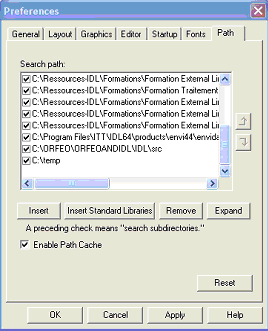
\includegraphics[width=7cm]{preferences.eps}
\caption{IDL Prefrences Window}
\end{center}
\end{figure}



\section{Testing from ENVI}
\begin{itemize}
    \item Launch ENVI and select from the main menu bar the \code{ORFEO Filters->Touzi edge detector} option.
    \item One of the GUIs \code{simpleENVIGui} or \code{simpleIDLGui} will appear depending on the \code{envi.men} text file contents. 
    \item Select the input and output files. 
    \item Enter a value in the \code{radius} field and press \code{OK}.
    \item The input file as well as the processed image should automatically appear in the ENVI  \code{Available Bands List}. 
          They can be displayed in standard ENVI windows(~\ref{bandlist} and ~\ref{viewer}).
\end{itemize}

\begin{figure}
    \begin{minipage}[b]{.46\linewidth}
        \centering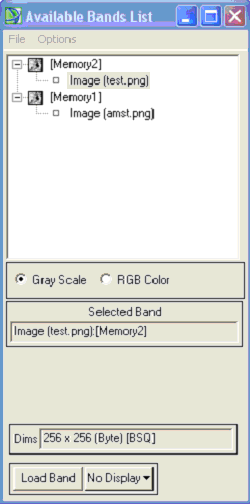
\includegraphics[width=5cm]{bandlist.eps}
        \caption{ Available Bands List ENVI window containing the input and output images}
        \label{bandlist}
    \end{minipage} \hfill
    \begin{minipage}[b]{.46\linewidth}
        \centering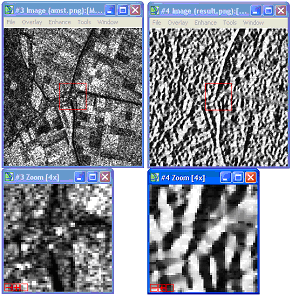
\includegraphics[width=8cm]{viewer.eps}
        \caption{Input (left) and Output (right)  examples of a Touzi filter}
        \label{viewer}
    \end{minipage}
\end{figure}

\section{Conclusion}
The integration of OTB routines into ENVI can be done by developing graphical user interfaces, either using only ENVI or using a mixed approach ENVI+IDL. 
The ENVI approach presents lots of advantages :
\begin{itemize}
    \item ENVI widgets are very simple to use, and don't require a deep IDL knowledge.
    \item Source code is very compact.
\end{itemize}

On the other hand, the ENVI+IDL approach is also interesting because it offers a wider widget choice, and allows a deeper widget control.
\\
As a conclusion, the use of the ENVI approach should be fully sufficient in simple cases, whereas The ENVI+IDL approach should be used in more complex situations as drawing images in draw widgets, or using specific widgets not directly available into ENVI.



\end{document}